\documentclass[conference]{IEEEtran}
\IEEEoverridecommandlockouts
% The preceding line is only needed to identify funding in the first footnote. If that is unneeded, please comment it out.
\usepackage{cite}
\usepackage{amsmath,amssymb,amsfonts}
\usepackage{algorithmic}
\usepackage{graphicx}
\usepackage{textcomp}
\usepackage{xcolor}
\def\BibTeX{{\rm B\kern-.05em{\sc i\kern-.025em b}\kern-.08em
    T\kern-.1667em\lower.7ex\hbox{E}\kern-.125emX}}
\begin{document}

\title{StarScope: Detecting Exoplanets from Stellar Light Curves\\
}

\makeatletter
\newcommand{\linebreakand}{%
  \end{@IEEEauthorhalign}
  \hfill\mbox{}\par
  \mbox{}\hfill\begin{@IEEEauthorhalign}
}
\makeatother
\author{\IEEEauthorblockN{Aarej Syed}
\IEEEauthorblockA{\textit{Erik Jonsson School of Engineering and Computer Science} \\
\textit{The University of Texas at Dallas}\\
Richardson, USA \\
aarej.syed@utdallas.edu}
\and
\IEEEauthorblockN{Van Nguyen}
\IEEEauthorblockA{\textit{Erik Jonsson School of Engineering and Computer Science} \\
\textit{The University of Texas at Dallas}\\
Richardson, USA \\
Van.Nguyen2@UTDallas.edu}
\linebreakand
\IEEEauthorblockN{Joshua Alvarado}
\IEEEauthorblockA{\textit{Erik Jonsson School of Engineering and Computer Science} \\
\textit{The University of Texas at Dallas}\\
Richardson, USA \\
Joshua.Alvarado@UTDallas.edu}
\and
\IEEEauthorblockN{Mohit Yadav Palam}
\IEEEauthorblockA{\textit{Erik Jonsson School of Engineering and Computer Science} \\
\textit{The University of Texas at Dallas}\\
Richardson, USA \\
MohitYadav.Palam@UTDallas.edu}
}

\maketitle

\begin{abstract}
This project explores how machine learning can be used to detect exoplanets from Kepler Space Telescope light curve data. Each star in the dataset is represented by 3197 flux measurements, which show how the star’s brightness changes over time. Since an exoplanet can cause small dips in brightness when it passes in front of a star, we used a one-dimensional convolutional neural network to learn these patterns and classify stars as either having or not having an exoplanet. The main parts of the CNN were implemented from scratch in Python using NumPy, including convolution, max pooling, dense layers, activation functions, weighted binary cross entropy, and backpropagation. Because the dataset contains many more non-exoplanet stars than exoplanet stars, weighted loss was used to help the model pay more attention to the rare exoplanet cases.
\end{abstract}

\begin{IEEEkeywords}
exoplanet detection, Kepler light curves, one-dimensional convolutional neural network
\end{IEEEkeywords}

\section{Introduction}
An exoplanet is a planet that revolves around a star outside the solar system. One way of discovering an exoplanet includes the analysis of light curves of stars. A light curve depicts the intensity of light emitted from a star over time. A planet passing between its star and an observer on Earth may block some amount of its light as it transits, resulting in sudden, regular dips in the flux of the star. These are known as transit dips.

For this task, we used a dataset of labeled light curves from the Kepler Space Telescope to classify stars into exoplanet-bearing and non-exoplanet-bearing stars \cite{kepler_dataset}. Every sample contains a light curve of 3197 evenly-spaced flux measurements, making a total of 3197 features arranged in one-dimensional sequence. The original dataset classifies a particular star into "no exoplanets" using the label 1, while the label 2 refers to a star with at least one exoplanet. However, within the Python script, the two classes are adjusted to be zero and one, so stars with no exoplanets constitute the negative class and stars with exoplanets constitute the positive class.

There is a lack of balance between the two classes since most stars in the dataset are not known to host exoplanets. Specifically, out of 5087 samples in the training set, 37 correspond to stars that host exoplanets, and out of 570 samples in the test set, only 5 correspond to stars that host exoplanets \cite{kepler_dataset}. In the training set, less than one percent of samples are of exoplanet-hosting stars, which means that any model that is reliable for this problem must be able to detect rare events, specifically transit dips.

Before any training is done, there are some preliminary tests such as verifying the dimensions of the data, type, number of missing values, and number of classes. It is also possible to plot light curves examples in each class. This helps us understand what distinguishes a sample with an exoplanet from one without.

For training purposes, we do an 80/20 split on the training set to produce a validation set; our dataset had the test set pre-split for us. Because of the class imbalance mentioned previously, we use stratified sampling to ensure that the training and validation sets had class ratios representative of the whole dataset.

Flux values are normalized using StandardScaler. During fitting of the scaler, only the training data is used. Then, the scaler is applied to the validation and test sets. This prevents data leakage. Next, normalization results are reshaped into the CNN format. Every sample will consist of 3197 time steps and 1 channel.

The one-dimensional convolutional neural network architecture suits this task well. Even though the features in each sample form a time series of flux measurements, recurrent neural networks such as long short-term memory networks are not suited for this task because they focus on time series \textit{prediction}. Exoplanets are identified by discovering recurring transit dips in a star's light curve, so we needed a model that could identify recurring transit dips. Convolutional neural networks, widely used in image processing, are useful for discovering \textit{spatial} patterns; since this problem involves identifying spatial patterns in the light curves, CNN is a natural fit. The network is capable of moving along the sequence of measurements and discovering local features such as drops in brightness. Such patterns will prove useful in differentiating between the two classes of stars. All core CNN modules were implemented from scratch using NumPy.

\section{Theoretical and Conceptual Study of the Model}

In this project, we use a 1D CNN to classify whether a star has at least one exoplanet from its light curve. Unlike the case of 2D CNNs in image processing applications, we treat the light curve in each sample as a one-dimensional time series and slide convolutional filters along the time axis to discover local patterns.

A light curve is just brightness over time. When a planet passes in front of a star, it creates a small transit dip; repeated transits of the exoplanet create short, periodic dips in the light curve, though the data is quite noisy. Instead of manually extracting features, we let the model learn patterns directly from the raw sequence.

Before training, the input is standardized using the training set to avoid data leakage.

We chose 1D CNN over RNN/LSTM because the task is mainly detecting local patterns in a fixed-length signal, not predicting future values. CNN is more suitable for this task since it can capture local patterns in the signal and is also simpler to train.

The model has a few main parts. Conv1D layers scan across the signal using sliding windows and try to detect local patterns. Each filter looks at a small part of the signal at a time, so it can pick up things like dips or small changes in shape, and computes the dot product of its kernel weights and the sliding window. The weights are initialized using a scaled random initialization (He initialization), which helps keep training stable at the beginning by preventing exploding signals with ReLU activations.

After that, we apply ReLU. It keeps positive values and sets negative values to zero, which introduces non-linearity. Then, max pooling reduces the size of the data by taking the maximum over small regions, which helps keep stronger signals while removing some noise. Max pooling also allows the model to detect recurring features in the light curve even if there are small shifts in position with each reoccurrence; this is relevant for exoplanet transit detection, because while they occur at regular intervals, they may not be perfectly spaced and the light curve is noisy to begin with.

After flattening, dense layers combine the extracted features and produce the final output. At the end, a sigmoid function is used so the output is between 0 and 1, which we interpret as a probability.

\subsection{Imbalanced Data}

The dataset is highly imbalanced (most samples are class 0). Because of that, accuracy can be misleading.

We use weighted binary cross-entropy:

\[
L = -\frac{1}{N} \sum_{i=1}^{N} w_i \left[ y_i \log(\hat{y}_i) + (1 - y_i)\log(1 - \hat{y}_i) \right]
\]

where $w_i = \text{pos\_weight}$ for the positive class, and $w_i = 1$ otherwise.

This makes the model pay more attention to the rare exoplanet cases. If the weight is too large, training can become unstable (gradients get large), so we tested a few values to balance this.

\subsection{Training}

We train the CNN for 10 epochs to balance greater insight into light curve features and model training time. For each epoch, we shuffle the dataset, which improves generalization by preventing the model from recognizing ordering artifacts in the dataset, such as all exoplanet samples being at the beginning of the dataset.

We train the model using mini-batches (batch size = 128), as this makes models efficient while keeping gradients stable. For each batch, we perform a forward pass, compute the loss, and then backpropagate gradients to update the weights.

In earlier runs, gradients were blowing up, so we added gradient clipping, and it helped make training more stable.

\subsection{Model Selection}

Because of the dataset's class imbalance, where the dataset is dominated by the majority class (no exoplanets), accuracy is not a reliable metric. We use F1 score instead, since it balances precision and recall, which is important when missing an exoplanet is costly.

The data is split into training, validation, and test sets. We select the best model based on validation F1, and the test set is only used at the end.

\section{Results and Analysis}

We ran four CNN models total. Our focus was to vary hyperparameters that were particularly relevant to our usage case. This is why we varied positive class weight and filter counts. Positive class weight is relevant because our dataset contains very few positive examples; therefore, it was important to find a positive class weight that made the model focus enough on predicting positive class examples correctly. Filter counts are relevant because they determine how many features and patterns each layer is able to detect; this is important for identifying transit dips in light curves.

In order to focus on the prior hyperparameters, we kept other hyperparameters constant:
\begin{itemize}
\item Layer count: 2. This allows the model to learn more complex features while keeping runtime relatively low.
\item Kernel size: 7 for first layer, 5 for second layer. This balances efficiency with a receptive field large enough to identify transit dips.
\item Learning rate: 0.0001. We chose this lower learning rate to prevent the problem of exploding gradients.
\item Batch size: 128. This batch size balances speed with generalization.
\item Training epochs: 10. We chose a moderate number of epochs that allowed the model to train for a sufficient amount of time while being time-efficient.
\end{itemize}

We chose specific values for the varied hyperparameters based on relevance to the problem. There were 5050 negative examples and 37 positive examples in the data, so the ratio of negative examples to positive examples was roughly 136.5. Therefore, we chose to test the values 100 and 150 for positive class weight, as these are lower and higher, respectively, than the negative-positive class ratio. For filter counts, we always used 32 for the second layer, but we switched between 16 and 32 for the first layer, as we wanted to see if this would increase the CNN's ability to learn more complex patterns.

\begin{figure}[t]
\centering
\footnotesize

\begin{verbatim}
EXPERIMENT 1

Parameters:
    Seed: 52
    Positive class weight: 100
    Filter counts: (16, 32)

Training time: 2631.23 s

Training:
class   precision  recall  f1-score  support
0       0.99       0.97    0.98      4039
1       0.04       0.17    0.06        30

Validation:
class   precision  recall  f1-score  support
0       0.99       0.97    0.98      1011
1       0.05       0.29    0.09         7


EXPERIMENT 2

Parameters:
    Seed: 53
    Positive class weight: 100
    Filter counts: (32, 32)

Training time: 4430.06 s

Training:
class   precision  recall  f1-score  support
0       0.99       0.98    0.99      4039
1       0.04       0.10    0.06        30

Validation:
class   precision  recall  f1-score  support
0       0.99       0.98    0.99      1011
1       0.00       0.00    0.00         7
\end{verbatim}

\caption{Training and validation results for Experiments 1–2.}
\label{fig:experiments_train_val_12}
\end{figure}

\begin{figure}[t]
\centering
\footnotesize

\begin{verbatim}
EXPERIMENT 3

Parameters:
    Seed: 54
    Positive class weight: 150
    Filter counts: (16, 32)

Training time: 2642.55 s

Training:
class   precision  recall  f1-score  support
0       0.99       0.91    0.95      4039
1       0.01       0.13    0.02        30

Validation:
class   precision  recall  f1-score  support
0       1.00       0.90    0.95      1011
1       0.03       0.43    0.05         7


EXPERIMENT 4

Parameters:
    Seed: 55
    Positive class weight: 150
    Filter counts: (32, 32)

Training time: 4736.10 s

Training:
class   precision  recall  f1-score  support
0       0.99       0.95    0.97      4039
1       0.03       0.23    0.06        30

Validation:
class   precision  recall  f1-score  support
0       0.99       0.93    0.96      1011
1       0.01       0.14    0.03         7
\end{verbatim}

\caption{Training and validation results for Experiments 3–4.}
\label{fig:experiments_train_val_34}
\end{figure}

\begin{figure}[t]
\centering
\footnotesize

\begin{verbatim}
TESTING (BEST EXPERIMENT: 1)

Hyperparameters: pos_weight=100, out_channels=(16, 32)
Validation F1 score: 0.0909

Testing:
class   precision  recall  f1-score  support
0       0.99       0.98    0.98       565
1       0.07       0.20    0.10         5
\end{verbatim}

\caption{Test set performance for the best CNN model (Experiment 1).}
\label{fig:test_results}
\end{figure}

Fig.~\ref{fig:experiments_train_val_12} and Fig.~\ref{fig:experiments_train_val_34} display the training and validation results of our experiments. Because examples with exoplanets are very rare in our dataset, we chose to use validation F1 score for the positive class (stars with exoplanets) as our criterion for what constitutes the best model. Therefore, overall accuracy, which was consistently high but was dominated by the negative class, was not included. Based on this criterion, experiment 1, with a positive class weight of 100 and a first-layer filter count of 16, is our best model, as it has a validation F1 score of 0.0909. However, this F1 score is very low. As mentioned previously, positive instances are very rare in our dataset, so it is difficult for the model to learn how to identify stars with exoplanets. This is also why, even when models cannot identify planets well, they still have high accuracy on paper.

Interestingly, increasing filter count does not seem to help performance. While experiment 1 resulted in the model being able to recall some positive examples, the model in experiment 2, which had a filter count of 32 in its first layer, predicted only class 0. Increasing positive class weight also does not seem to help performance; in experiment 3, which has a positive class weight of 150, the model has validation precision for the positive class of only 0.03 but also has validation recall for the positive class of 0.43. This indicates that even though higher class weight makes the model predict a star has exoplanets more often, it does not improve identification of exoplanet-bearing stars because the model increases its positive predictions without learning how to differentiate true positives from false positives.

\begin{figure}[t]
\centering
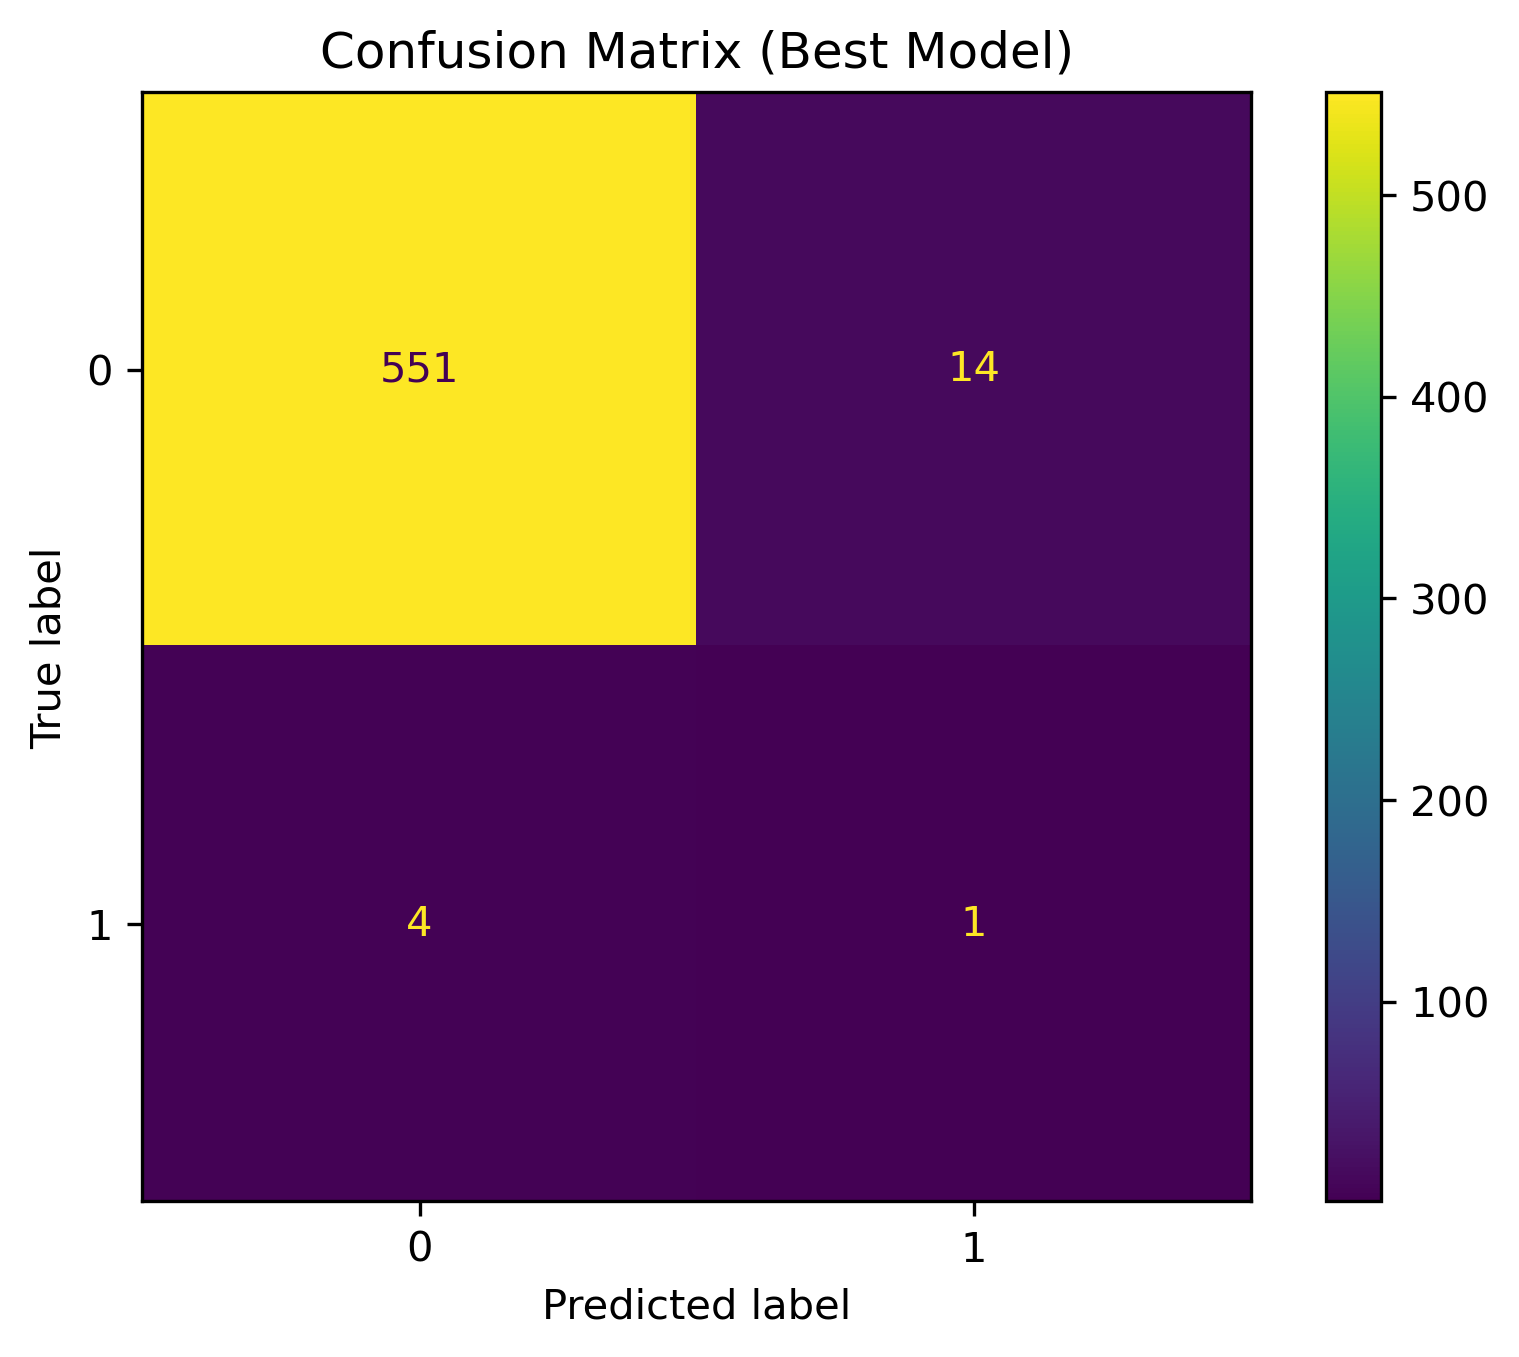
\includegraphics[width=0.85\columnwidth]{confusion_matrix.png}
\caption{Confusion matrix for the best model on the test set.}
\label{fig:confusion}
\end{figure}

Fig. ~\ref{fig:confusion} displays the confusion matrix for the best model after being tested with the testing data split; detailed results from this test are shown in Fig. ~\ref{fig:test_results}. According to the confusion matrix, out of 15 positive predictions, one was an exoplanet-bearing star and the others were stars with no exoplanets, yielding a precision of approximately 0.067. This means that the model from experiment 1 significantly over-predicts stars with exoplanets. Additionally, out of 5 true positive examples in the testing data split, 4 were incorrectly predicted to have no exoplanets, yielding a recall of 0.2. While the model's correct classification of 1 positive example shows that it has slight predictive power, it fails to detect exoplanets reliably.

\begin{figure}[t]
\centering
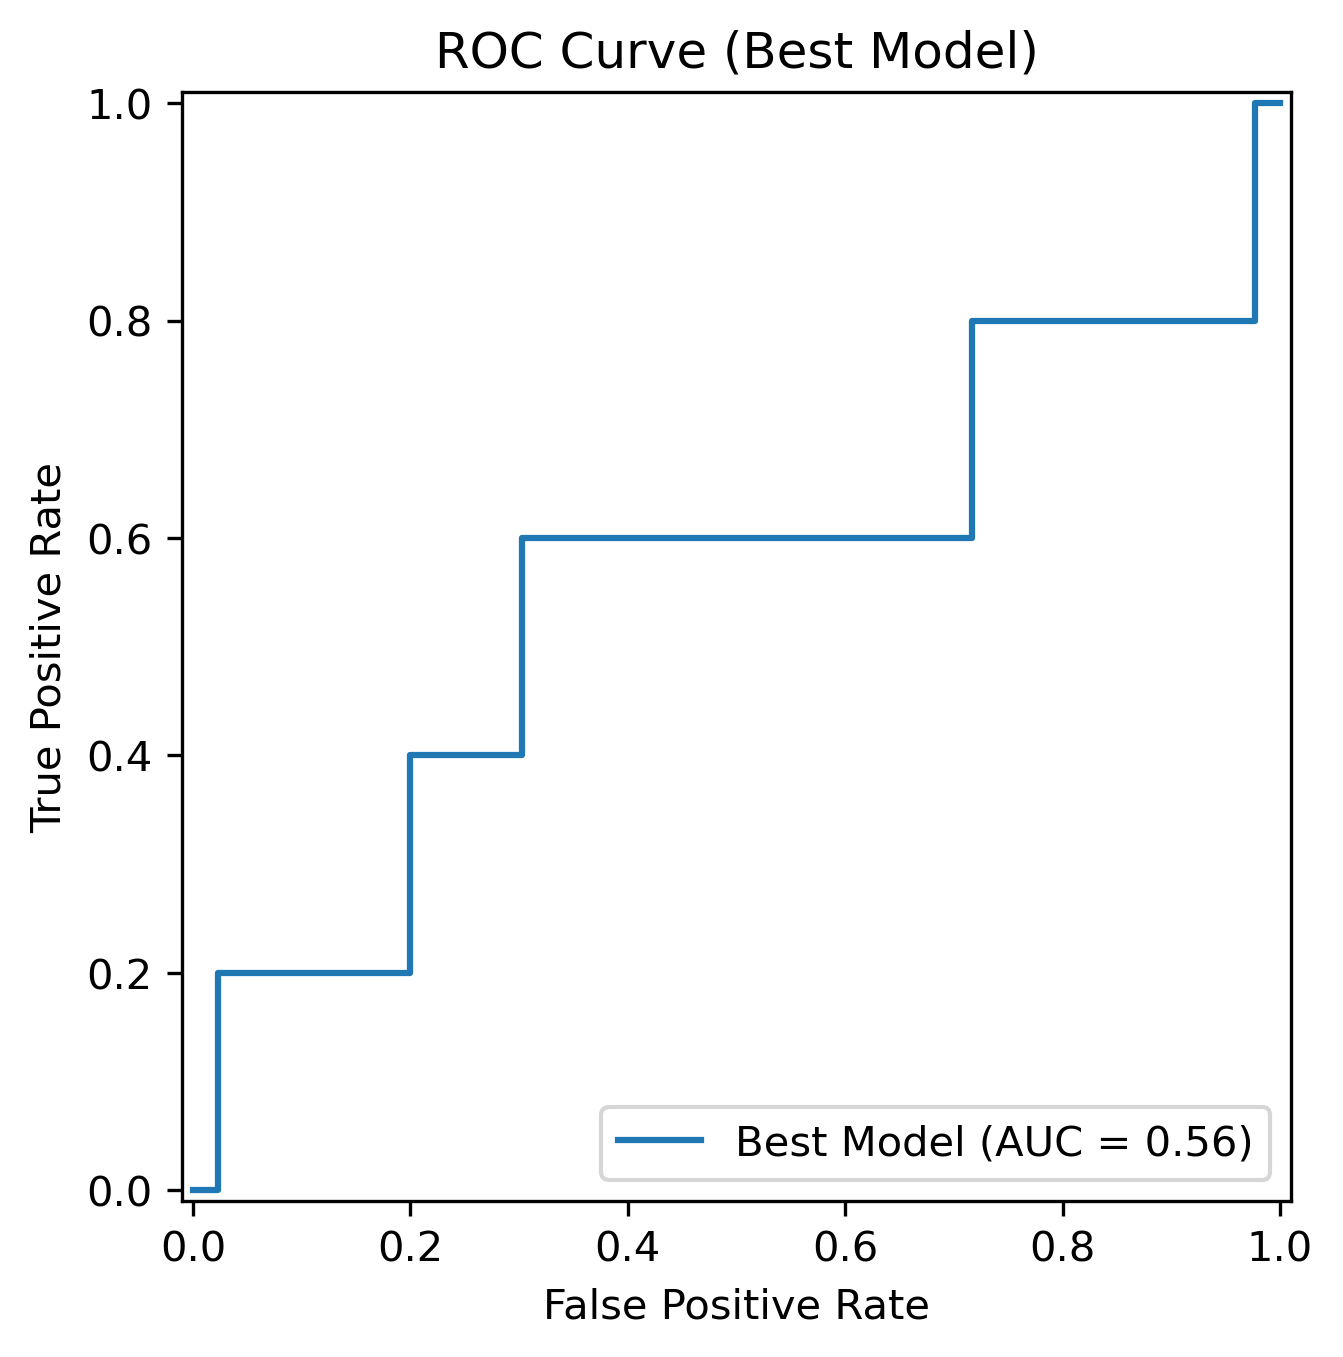
\includegraphics[width=0.85\columnwidth]{roc_curve.png}
\caption{ROC curve for the best model on the test set (AUC = 0.56).}
\label{fig:roc}
\end{figure}

Fig. ~\ref{fig:roc} depicts the ROC curve for the best model. The area under the curve (AUC) is 0.56, which is only slightly better than random guessing (AUC = 0.5). This means that across different classification thresholds, the model has an existing, but very limited, ability to differentiate between stars with and without exoplanets. Furthermore, changing the classification threshold from its default of 0.5 does not significantly increase the model's ability to discriminate between positive and negative classes. This further confirms our findings from the confusion matrix that the model struggles to learn how to detect transit dips, so it cannot develop a generalized ability to detect exoplanets.

Changes to hyperparameters do not significantly improve the models' abilities to correctly identify stars with exoplanets. Additionally, the low AUC, along with the previously observed low F1 score and recall for the positive class, illustrates that the main limitation is the severe class imbalance in the dataset; the model's performance is constrained by the rarity of positive class instances. Overall, our results suggest data imbalance, not hyperparameter choice, is what limits model performance here.

\section{Conclusion and Future Work}

We implemented a 1D convolutional neural network from scratch to predict whether stars have exoplanets or not based on light curves collected by the Kepler Space Telescope. As our dataset was heavily biased towards stars with no exoplanets, we used F1 score for the positive class, rather than overall accuracy, to determine which model was best suited for the task. Although the model achieved high overall accuracy, it consistently performed poorly on predicting stars with exoplanets, thus leading to low F1 scores for the positive class. Neither increasing the model's capacity to learn complex patterns nor changing positive class weight significantly improved the detection of stars with exoplanets. As shown by the experiment results and the confusion matrix for the best model's testing set performance, the model predicts stars without exoplanets, the majority class, very well, but is unable to learn how to reliably identify the rare exoplanet-bearing stars. Overall, the model's poor performance in identifying stars with exoplanets is not a result of the model's parameters but arises from an inherent limitation in the dataset: its severe class imbalance.

Future work would focus on addressing the class imbalance to ensure that the model can adequately learn the positive class. Suggested methods for addressing this class imbalance would be random oversampling, which artificially increases the number of positive class samples, and/or changing the scope of the task from detecting stars with exoplanets to detecting light curve anomalies that may indicate exoplanet presence and should be reviewed by humans.

\begin{thebibliography}{00}
\bibitem{kepler_dataset} KeplersMachines, ``Exoplanet Hunting in Deep Space,'' Kaggle dataset. [Online]. Available: https://www.kaggle.com/datasets/keplersmachines/kepler-labelled-time-series-data. [Accessed: May 4, 2026].
\end{thebibliography}

\end{document}
